\documentclass[12pt,a4paper]{article}
\usepackage[utf8]{inputenc}
\usepackage[spanish]{babel}
\usepackage{amsmath}
\usepackage{amsfonts}
\usepackage{amssymb}
\usepackage{graphicx}
\usepackage[left=2cm,right=2cm,top=2cm,bottom=2cm]{geometry}

\usepackage{enumitem}
\usepackage{algorithm}
\usepackage{algorithmic}
\usepackage[hidelinks]{hyperref}

\usepackage{subcaption}
\usepackage{pgfplots}


\author{Ignacio Aguilera Martos}
\title{Práctica 1 \\ Aprendizaje Automático}
\date{25 de Marzo de 2019}

\setlength{\parindent}{0cm}
\setlength{\parskip}{10px}


\begin{document}
	\maketitle

	\tableofcontents

	\newpage

\section{Ejercicio 1}

\subsection{Apartado 1}

Se nos pide implementar el algoritmo de gradiente descendente, veamos como funciona para justificar la implementación.

El algoritmo de gradiente descendente aplicado a minimización de funciones toma la idea del ajuste de una función lineal que hemos estudiado en teoría. Ahora en vez de actualizar $w_j$ de forma proporcional a la derivada parcial j-ésima de el error dentro de la muestra vamos a actualizarla mediante la derivada parcial j-ésima de la función que queremos minimizar.

El algoritmo parte de un punto $w$ inicial, que se irá actualizando hasta aproximar el mínimo de la función. El valor de $w$ en la iteración i+1-ésima será el valor de $w$ en la iteración i-ésima menos una constante de proporcionalidad que llamamos tasa de aprendizaje por el gradiente de la función a minimizar, esto es:

$$w_{i+1} = w_i - \eta \cdot \nabla f(x_1,...,x_n)$$

Donde $f(x_1,...,x_n)$ es la función que queremos minimizar.

De esta forma lo que vamos a hacer en la práctica es comprobar lo siguiente: vamos a actualizar de esta forma el valor de $w$ hasta que agotemos un número de iteraciones máximas fijadas o hasta que el valor absoluto de la diferencia de $f(w_i))$ y $f(w_{i+1})$ sea menor que una cierta tolerancia, esto es que la imagen de los $w_i$ y $w_{i+1}$ no hayan experimentado un cambio apreciable entre dos iteraciones consecutivas.

Cabe destacar que en mi caso he generalizado la implementación del algoritmo mediante el uso de la librería SymPy. Mediante esta librería he implementado una función que generaliza el cálculo del gradiente en un punto, de tal forma que no tengo que programar explícitamente la función que calcula el gradiente de la función que queremos minimizar. Esto se plasma en las funciones ``evaluate'' y ``gradiente'' de mi código.

\subsection{Apartado 2}

\subsubsection{Apartado a}

En este apartado se nos proporciona la siguiente función a minimizar:

$$E(u,v) = (u^2 e^{v} - 2v^2 e^{-u})^2$$

Vamos a calcular analíticamente la expresión del gradiente como se nos pide en el ejercicio. Lo primero que tenemos que hacer es ver cómo sería la expresión del gradiente en nuestro caso:

$$\nabla E(u,v) = (\frac{\partial E(u,v)}{\partial u},\frac{\partial E(u,v)}{\partial v})$$

Calculemos pues cada una de las dos parciales.

$$\frac{\partial E(u,v)}{\partial u} = 2(u^2 e^{v} - 2v^2 e^{-u})(2ue^{v}+2v^2e^{-u})$$

$$\frac{\partial E(u,v)}{\partial v} = 2(u^2 e^{v} - 2v^2 e^{-u})(u^2 e^{v}-4ve^{-u})$$

Por tanto:

$$\nabla E(u,v) = (\frac{\partial E(u,v)}{\partial u},\frac{\partial E(u,v)}{\partial v}) = 2 (u^2 e^{v} - 2v^2 e^{-u})\cdot [(2ue^{v}+2v^2e^{-u}), (u^2 e^{v}-4ve^{-u})](u,v)$$

Cabe decir que esta es una función $\nabla E(u,v): \mathbb{R}^2 \rightarrow \mathbb{R}^2$, es decir que toma dos variables y que obtiene un vector de dimensión 2.

\subsubsection{Apartado b y c}

En este apartado se nos pide dar el punto en el que el método de gradiente descendente ha alcanzado por primera vez un valor de la función menor que $10^{-14}$ y el número de iteraciones que ha consumido hasta obtener dicho valor.

En este caso el punto en el que se ha encontrado un valor que cumple esta restricción es $w=(0.619207678450638,0.968448269010049)$ y para ello ha consumido $33$ iteraciones.

\subsection{Apartado 3}

Consideramos en este apartado la función:

$$f(x,y) = x^2 + 2y^2 + 2\sin{(2\pi x)}\sin{(2\pi y)}$$

\subsubsection{Apartado a}

Se nos pide aplicar el algoritmo de gradiente descendente a la función anteriormente definida empezando en el punto $(x_0 = 0.1, y_0 = 0.1)$ con tasa de aprendizaje $\eta = 0.01$ y como máximo $50$ iteraciones.

Tras esto se nos pide elaborar un gráfico con los valores de la función obtenidos para cada iteración. Veamos los gráficos para poder analizarlos.

\begin{figure}[H]
	\centering
	\begin{subfigure}{0.45\textwidth}
		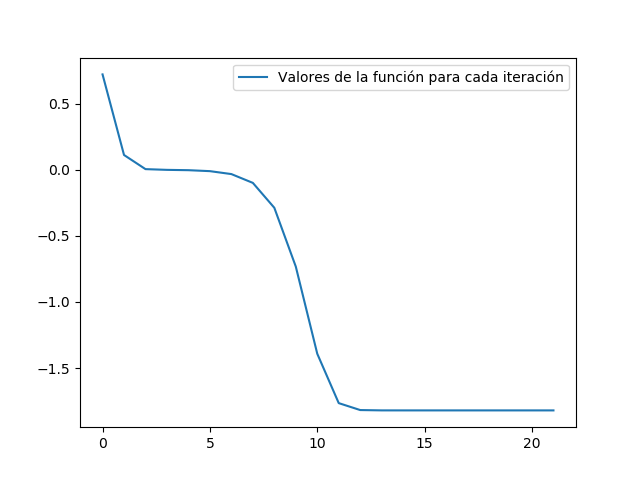
\includegraphics[scale=0.5]{./Imagenes/3a1.png}
		\caption{Tasa de aprendizaje $\eta=0.01$}
		\label{3a1}
	\end{subfigure}
	\begin{subfigure}{0.45\textwidth}
		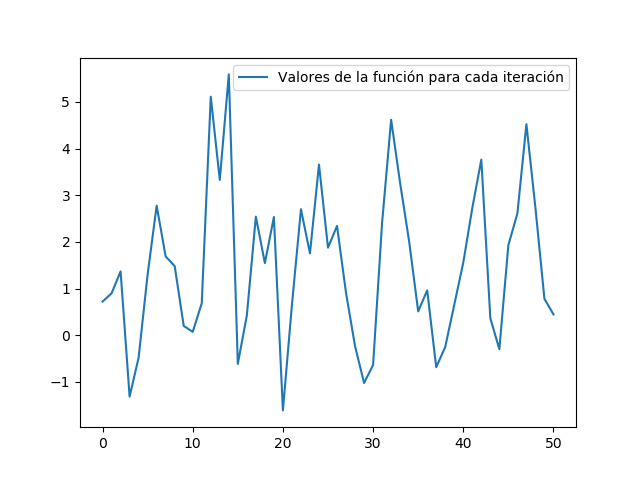
\includegraphics[scale=0.5]{./Imagenes/3a2.png}
		\caption{Tasa de aprendizaje $\eta=0.1$}
		\label{3a2}
	\end{subfigure}
\end{figure}

Como podemos observar el resultado usando $\eta=0.01$ siempre mejora en cada iteración, o a lo sumo permanece en un valor igual, en cambio con $\eta=0.1$ obtenemos una oscilación pronunciada entre iteraciones, esto es, entre dos iteraciones consecutivas no siempre pasamos a un punto con menor valor de la función, si no que mejoramos y empeoramos el resultado de forma cíclica.

Cabe explicar este comportamiento de forma más detallada para razonarlo. La tasa de aprendizaje nos da el factor de salto por el que va multiplicado el gradiente de la función, es decir, a mayor tasa de aprendizaje mayor será el salto que hagamos para obtener el siguiente valor de $w$. Supongamos que tenemos una función como $f(x)=x^2$:

\begin{figure}[H]
	\centering
	\begin{tikzpicture}
		\begin{axis}[ 
			xlabel=$x$,
			ylabel={$f(x) = x^2$}
			] 
			\addplot[blue,thick](x,x^2); 
		\end{axis}
	\end{tikzpicture}
\end{figure}

Según el valor de la tasa de aprendizaje $\eta$ podemos encontrarnos con los dos escenarios que nos están ocurriendo:

\begin{figure}[H]
	\begin{subfigure}{0.45\textwidth}
		\centering
		\begin{tikzpicture}
			\begin{axis}[ 
				xlabel=$x$,
				ylabel={$f(x) = x^2$}
				] 
				\addplot[blue,thick](x,x^2);
				\addplot+ [mark=*] table{
					0 0
					-2 4
					-4 16
				};
			\end{axis}
		\end{tikzpicture}
	\end{subfigure}
	\begin{subfigure}{0.45\textwidth}
		\centering
		\begin{tikzpicture}
		\begin{axis}[ 
		xlabel=$x$,
		ylabel={$f(x) = x^2$}
		] 
		\addplot[blue,thick](x,x^2);
		\addplot+ [mark=*] table{
			0 0
			1 1
			-1 1
			2 4
			-2 4
			3 9
			-3 9
			4 16
			-4 16
		};
		\end{axis}
		\end{tikzpicture}
	\end{subfigure}
	\caption{Ejemplo de comportamiento del gradiente descendente}
	\label{descripcionEta}
\end{figure}

Como podemos ver una aproximación no realiza ``saltos'' alrededor del mínimo, si no que va de forma directa al mínimo, mientras que en el otro caso tenemos una oscilación alrededor del mínimo. 

Si estudiamos la dependencia del comportamiento del algoritmo en función de la tasa de aprendizaje $\eta$ vemos que la magnitud del salto del punto actual al siguiente viene dada exactamente por $\eta$ en la dirección del gradiente de la función.

En nuestro caso, con $\eta = 0.01$ podemos osbervar en la gráfica \textbf{\ref{3a1}} que la convergencia es de forma gradual y sin saltos alrededor del mínimo, pues siempre que se progresa en cada iteración se hace obteniendo un valor menor de la función, es decir estaríamos en el primero de los casos expuestos de la figura \textbf{\ref{descripcionEta}}.

En el segundo caso con $\eta=0.1$ podemos observar en la gráfica \textbf{\ref{3a2}} que el comportamiento es errático. Si observamos la evolución entre iteraciones podemos observar que no mejora si no que oscila alrededor del mínimo sin llegar a él. Esto es debido a que la longitud del salto, es decir, el valor de $\eta$ es demasiado grande y hace que avance demasiado entre iteraciones. Esto comparado con nuestro ejemplo de la figura \textbf{\ref{descripcionEta}} se correspondería con el segundo de los casos, en el que el camino hacia el mínimo de la función se hace oscilando entorno a él.

En la figura con $\eta=0.1$ también se aprecia que la amplitud de valores que toma va disminuyendo, es decir, poco a poco se está dirigiendo hacia el mínimo. El algoritmo gradiente descendente llegará eventualmente al mínimo con este valor de $\eta$ pero consumirá un número mucho mayor de iteraciones que si escogemos de forma más ajustada la tasa de aprendizaje.

Esto último mencionado no quiere decir que el algoritmo partiendo de un punto inicial fijo siempre converja hacia el mismo mínimo de la función, ya que puede que en función del valor de $\eta$ las iteraciones vayan saltando hasta dar con otro mínimo local o global de la función.

\end{document}
